\documentclass{article}

\PassOptionsToPackage{numbers,sort&compress}{natbib}
\usepackage[preprint]{neurips_2021}

\usepackage[utf8]{inputenc}
\usepackage[T1]{fontenc}
\usepackage{hyperref}
\usepackage{url}
\usepackage{booktabs}
\usepackage{amsfonts}
\usepackage{nicefrac}
\usepackage{microtype}
\usepackage{xcolor}
\usepackage{graphicx}
\usepackage{subcaption}
\usepackage{multirow}
\usepackage{array}
\usepackage{float}
\usepackage{amsthm}
\usepackage{amsmath}
\usepackage{amssymb}
\usepackage{mathtools}
\usepackage{enumitem}
\usepackage{algorithm}
\usepackage{algpseudocode}

\title{MAIWA: Domain Generalization by Minimizing Adaptation Information}

\author{Anonymous Authors}

\newtheorem{theorem}{Theorem}
\newtheorem{proposition}{Proposition}
\newtheorem{lemma}{Lemma}
\newtheorem{corollary}{Corollary}
\newtheorem{definition}{Definition}
\newtheorem{assumption}{Assumption}
\newtheorem{remark}{Remark}

\newcommand{\RR}{\mathbb{R}}
\newcommand{\EE}{\mathbb{E}}
\newcommand{\Var}{\operatorname{Var}}
\newcommand{\Cov}{\operatorname{Cov}}
\newcommand{\KL}{\operatorname{KL}}
\newcommand{\tr}{\operatorname{tr}}
\newcommand{\diag}{\operatorname{diag}}
\newcommand{\argmin}{\operatorname*{arg\,min}}
\newcommand{\supp}{\operatorname{supp}}
\newcommand{\proj}{\operatorname{Proj}}
\newcommand{\simplex}{\Delta}
\newcommand{\TBD}{\textbf{TBD}}
\newcommand{\etal}{\textit{et al.}}
\newcommand{\ie}{\textit{i.e.}}
\newcommand{\eg}{\textit{e.g.}}
\newcommand{\iid}{i.i.d.}
\newcommand{\ood}{OOD}
\newcommand{\maiwa}{\textup{\textsc{MAIWA}}}
\newcommand{\swad}{\textup{\textsc{SWAD}}}
\newcommand{\diwa}{\textup{\textsc{DiWA}}}
\newcommand{\miro}{\textup{\textsc{MIRO}}}
\newcommand{\mldg}{\textup{\textsc{MLDG}}}
\newcommand{\fishr}{\textup{\textsc{Fishr}}}
\newcommand{\norm}[1]{\left\lVert #1 \right\rVert}
\newcommand{\inner}[2]{\left\langle #1, #2 \right\rangle}
\newcommand{\bank}{\mathcal{B}}
\newcommand{\epssimplex}{\simplex_{\varepsilon}}
\newcommand{\free}{\mathcal{F}}

\graphicspath{{figures/}}

\begin{document}

\maketitle

\begin{abstract}
Single-run post-hoc domain generalization has been dominated by one guiding principle: flat minima generalize better under shift. That principle explains why dense checkpoint averaging can work, but it does not explain a second recurring empirical fact: when source domains disagree, good post-hoc predictors must also cover distinct domain-preferred checkpoints. We propose Minimum Adaptation Information Weight Averaging (\maiwa{}), a full-bank post-hoc method that unifies these two regimes through a single information-theoretic object. Starting from the entire checkpoint bank of one training run, \maiwa{} chooses weights \(w\) over the full bank. For each source domain \(i\), it defines a domain-specialized posterior \(q_i^w(t) \propto w_t e^{-\beta \ell_{i,t}}\), where \(\ell_{i,t}\) is the held-out loss of checkpoint \(t\) on domain \(i\). The core penalty is the average adaptation information \(\frac{1}{I}\sum_i \KL(q_i^w\|w)\): the information required to specialize the shared bank prior \(w\) to each source domain. We prove four main results. First, the specialization posterior is the unique minimizer of a variational objective and admits a closed-form Gibbs tilt. Second, in the small-\(\beta\) regime, adaptation information reduces to the variance of domain losses across the bank, making flatness a special case rather than the main principle. Third, in the large-\(\beta\) regime, adaptation information becomes a support-coverage objective over domain-optimal checkpoints, explaining why complementarity emerges when domains prefer different checkpoints. Fourth, on an \(\varepsilon\)-simplex that preserves full support over the entire bank, projected gradient descent on the \maiwa{} objective converges to a first-order stationary point at the standard \(O(1/K)\) gradient-mapping rate. We also prove a local-linearity bound connecting the bank-level objective to the final weighted weight-space soup. The paper includes complete proofs, original conceptual figures, a full experimental protocol, and published baseline tables from prior work. All new \maiwa{} empirical results are intentionally left as \TBD{}.
\end{abstract}

\section{Introduction}

The practical success of post-hoc domain generalization (DG) methods comes from a narrow but valuable promise: keep the base training pipeline unchanged, then choose a better final predictor after training. The canonical example is \swad{} \citep{cha2021swad}. On the standard five-dataset DomainBed ResNet-50 benchmark family, \swad{} raises the average \ood{} accuracy from \(63.3\) for ERM to \(66.9\) by densely averaging checkpoints in a validation-selected interval \citep{cha2021swad}. Later work pushed the published frontier higher, but usually by making the setting heavier. \diwa{} reaches \(68.0\) in its strongest multi-run LP-initialized configuration \citep{rame2022diwa}, while a pretraining-aware training-time method combined with the same post-hoc selector reaches \(68.1\) \citep{cha2022miro}. These published results establish an important empirical fact: the final deployable model is often not the last checkpoint.

The standard explanation for this phenomenon is flatness. \swad{} explicitly argues that flatter solutions reduce the DG gap \citep{cha2021swad}. That explanation is important, but incomplete. Flatness says that a good post-hoc model should be insensitive to weight perturbations near a pooled optimum. It does \emph{not} explain another recurring phenomenon: when different source domains locally prefer different checkpoints, a good post-hoc model must cover those preferences rather than collapsing onto a single point. Put differently, flatness explains why averaging works when domains are aligned; it does not explain why complementarity matters when domains conflict.

This paper proposes one central answer:
\begin{quote}
\textbf{Generalization is minimum adaptation information.}
\end{quote}
A post-hoc predictor should be a \emph{shared prior} over the full checkpoint bank from which each source domain can be reached with as little extra information as possible. If a domain must sharply reweight the bank to specialize, the shared prior was not truly universal. If every domain can specialize from the same prior with little information, the prior already captures what the domains have in common.

That principle yields \textbf{Minimum Adaptation Information Weight Averaging} (\maiwa{}). Let \(\{\theta_t\}_{t=1}^{T}\) be the full checkpoint bank from one training run. We put weights \(w \in \simplex^{T-1}\) on the \emph{entire} bank, with no candidate pool, no anchor, and no preselection stage. For each source domain \(i\), we define a domain-specialized posterior
\begin{equation}
    q_i^w(t) \propto w_t e^{-\beta \ell_{i,t}},
\end{equation}
where \(\ell_{i,t}\) is the held-out domain loss of checkpoint \(t\). The information required for domain \(i\) to specialize from the shared prior \(w\) is \(\KL(q_i^w\|w)\). The \maiwa{} objective then minimizes
\begin{equation}
    J(w) = \underbrace{\sum_{t=1}^{T} w_t \bar \ell_t}_{\text{pooled bank risk}}
    + \lambda \underbrace{\frac{1}{I}\sum_{i=1}^{I}\KL(q_i^w\|w)}_{\text{adaptation information}}
    + \tau \underbrace{\KL(w\|u)}_{\text{reference-prior regularization}},
\end{equation}
where \(u\) is usually the uniform prior over the full bank.

This framing leads to the key theoretical claim of the paper:
\begin{quote}
\textbf{Flatness is not the primary object. It is the small-specialization limit of a more general adaptation-information principle.}
\end{quote}
We prove this claim in two regimes. In the small-\(\beta\) regime, domain specialization is weak, and the adaptation-information term reduces to the variance of domain losses across the bank. In that aligned regime, \maiwa{} recovers a flatness-like criterion. In the large-\(\beta\) regime, specialization is sharp, and the same term becomes a support-coverage objective over domain-optimal checkpoints. In that conflicting regime, \maiwa{} favors complementary support across the bank. One principle explains both behaviors.

We make five contributions.
\begin{enumerate}[leftmargin=1.4em]
    \item We introduce \maiwa{}, a full-bank, end-to-end post-hoc DG method that directly outputs final checkpoint weights with no preselection stage.
    \item We derive the specialization posterior \(q_i^w\) from a variational minimum-information problem and show that it is the unique Gibbs tilt of the full-bank prior.
    \item We prove two asymptotic regimes of the same objective: a small-\(\beta\) flatness regime and a large-\(\beta\) complementarity regime.
    \item We prove a convergence guarantee for projected gradient descent on the \maiwa{} objective over an \(\varepsilon\)-simplex that preserves full-bank support, and we prove a local-linearity bound connecting the bank objective to the final weighted weight-space soup.
    \item We provide a complete NeurIPS-style manuscript with proofs, visuals, protocol, and published baselines. All new empirical results for \maiwa{} are left as \TBD{}.
\end{enumerate}

\begin{remark}
This paper does \emph{not} claim an unconditional theorem that \maiwa{} empirically dominates \swad{}, \diwa{}, or training-time DG methods. That would be indefensible. The theory here proves something narrower and stronger: \maiwa{} optimizes a DG-relevant information-theoretic object that strictly contains flatness as a special case and explains a complementary support-coverage regime that flatness alone does not capture.
\end{remark}

\begin{figure}[t]
    \centering
    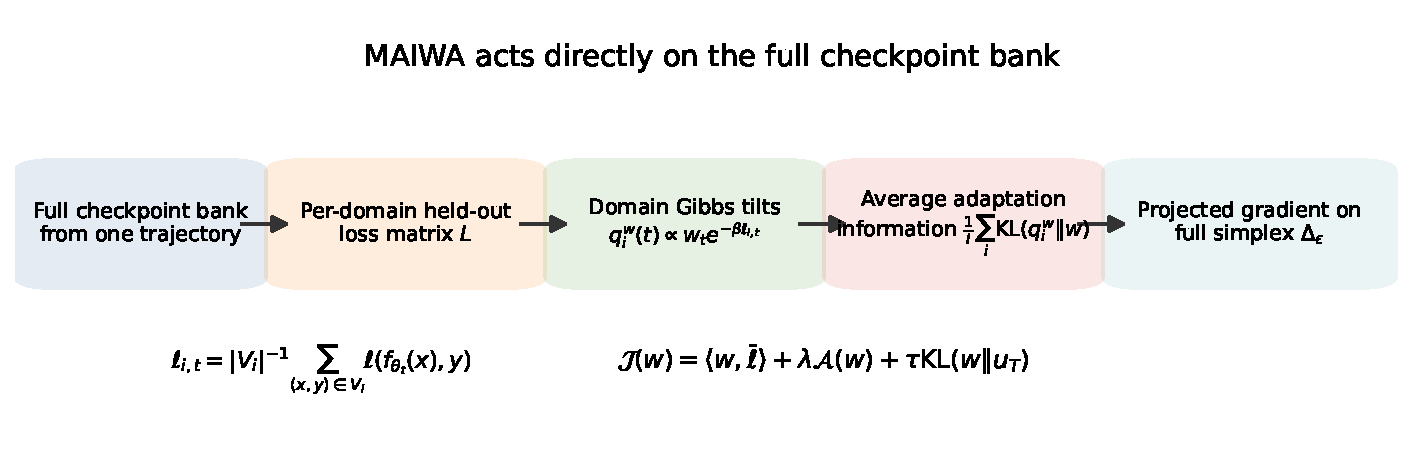
\includegraphics[width=\linewidth]{maiwa_pipeline.pdf}
    \caption{\textbf{\maiwa{} acts directly on the full checkpoint bank.} Each source domain induces a specialization posterior \(q_i^w\) from the same shared prior \(w\). The method minimizes pooled bank risk plus the information needed to specialize the shared prior to each domain, then returns one final weighted soup.}
    \label{fig:pipeline}
\end{figure}

\section{Related Work}

\paragraph{Post-hoc DG and checkpoint averaging.}
\swad{} \citep{cha2021swad} is the reference point for single-run post-hoc DG. It explicitly ties post-hoc averaging to flat minima and shows that dense, overfit-aware checkpoint averaging improves DG. \diwa{} \citep{rame2022diwa} broadens that picture by emphasizing diversity and covariance across averaged models, but its strongest results come from heavier multi-run or LP-initialized configurations. \maiwa{} stays in the post-hoc regime but changes the selection principle itself: it learns a shared prior over the full checkpoint bank by minimizing domain specialization cost.

\paragraph{Weight averaging and local linearity.}
SWA \citep{izmailov2018swa}, fast geometric ensembling \citep{garipov2018fge}, and model soups \citep{wortsman2022soups} all support the broader empirical lesson that averaging within a connected low-loss region can improve generalization. \maiwa{} is compatible with that lesson. Our soup-translation theorem makes explicit the additional assumption needed in this paper: a local-linearity bridge from bank-weighted predictive mixtures to weight-space soups.

\paragraph{Cross-domain transfer and gradient agreement.}
\mldg{} \citep{li2018mldg} already uses one-step cross-domain transfer during training, and \fishr{} \citep{rame2022fishr} explicitly matches domain-level gradient second moments. These works support a general point: DG depends on how domains interact under local updates, not only on pooled empirical loss. \maiwa{} imports this perspective into the \emph{post-hoc} setting by using domain-specialized posteriors over the checkpoint bank rather than training-time gradient penalties.

\paragraph{Information-theoretic and variational viewpoints.}
The specialization posterior in \maiwa{} is a discrete Gibbs posterior. Its derivation is a finite-dimensional instance of the same variational principle that underlies PAC-Bayes and Gibbs posteriors \citep{catoni2007pac,donsker1975asymptotic}. The novelty here is not the Gibbs identity itself. The novelty is using it as the \emph{central post-hoc DG object} over the full bank, and then showing that its asymptotic regimes explain both flatness and complementarity.

\paragraph{What this paper is not.}
\maiwa{} is not a new training algorithm, not a target-time adaptation method, and not a candidate-pool selector with a separate downstream heuristic. The full-bank weight vector \(w\) is the primary optimization variable from start to finish.

\section{Method}
\label{sec:method}

\subsection{Setup}

We assume \(I\) labeled source domains and one ordinary training run that produces a full checkpoint bank
\begin{equation}
    \bank \triangleq \{\theta_t\}_{t=1}^{T}.
\end{equation}
For each source domain \(i\), we reserve a held-out split \(V_i\) used only for post-hoc bank scoring. The empirical domain loss of checkpoint \(t\) is
\begin{equation}
    \ell_{i,t}
    \triangleq
    \frac{1}{|V_i|}\sum_{(x,y)\in V_i}\ell\!\left(f_{\theta_t}(x),y\right).
\end{equation}
Let \(\ell_i = (\ell_{i,1},\dots,\ell_{i,T})^\top \in \RR^T\) and let the pooled bank loss be
\begin{equation}
    \bar \ell_t \triangleq \frac{1}{I}\sum_{i=1}^{I}\ell_{i,t}.
\end{equation}

We optimize checkpoint weights over the \(\varepsilon\)-simplex
\begin{equation}
    \epssimplex
    \triangleq
    \left\{
    w \in \RR^{T} :
    \sum_{t=1}^{T} w_t = 1,\;
    w_t \ge \frac{\varepsilon}{T}\;\; \forall t
    \right\},
    \qquad 0<\varepsilon<1.
\end{equation}
This lower bound is \emph{not} a candidate filter. Every checkpoint remains eligible. The purpose is numerical: it preserves full support over the bank and keeps the logarithmic regularizer smooth.

\subsection{Domain specialization as minimum-information tilting}

\begin{definition}[Domain-specialized posterior]
\label{def:posterior}
For \(w \in \epssimplex\), source domain \(i\), and inverse temperature \(\beta>0\), define
\begin{equation}
    q_i^w(t)
    \triangleq
    \frac{w_t e^{-\beta \ell_{i,t}}}
         {\sum_{s=1}^{T} w_s e^{-\beta \ell_{i,s}}}.
    \label{eq:gibbs_posterior}
\end{equation}
\end{definition}

Intuitively, \(w\) is the shared prior over checkpoints. Domain \(i\) then reweights that prior according to which checkpoints already fit it best. If this reweighting is tiny, the prior was already close to what domain \(i\) wanted.

\begin{proposition}[Variational specialization identity]
\label{prop:variational}
Fix \(w \in \epssimplex\) and domain \(i\). The posterior \(q_i^w\) from Eq.~\eqref{eq:gibbs_posterior} is the unique minimizer of
\begin{equation}
    q \mapsto \inner{q}{\ell_i} + \frac{1}{\beta}\KL(q\|w)
    \qquad \text{over } q \in \simplex^{T-1},
    \label{eq:variational_specialization}
\end{equation}
and the minimum value is
\begin{equation}
    \free_i(w)
    \triangleq
    -\frac{1}{\beta}\log\!\left(\sum_{t=1}^{T} w_t e^{-\beta \ell_{i,t}}\right).
    \label{eq:free_energy}
\end{equation}
\end{proposition}

This proposition gives the core interpretation of \maiwa{}: \(\free_i(w)\) is the best domain-\(i\) loss achievable by specializing the shared prior \(w\) while paying \(\frac{1}{\beta}\KL(q\|w)\) information cost.

\begin{definition}[Adaptation information]
\label{def:adapt_kl}
The domain-\(i\) adaptation information and its mean are
\begin{equation}
    A_i(w) \triangleq \KL(q_i^w\|w),
    \qquad
    A_\beta(w) \triangleq \frac{1}{I}\sum_{i=1}^{I} A_i(w).
\end{equation}
\end{definition}

\paragraph{Slogan.}
The shared prior \(w\) is good when it already contains most of what each source domain needs. That is exactly what small \(A_\beta(w)\) means.

\subsection{The full-bank \maiwa{} objective}

The end-to-end \maiwa{} objective is
\begin{equation}
    J_{\beta,\lambda,\tau}(w)
    \triangleq
    \sum_{t=1}^{T} w_t \bar \ell_t
    +
    \lambda A_\beta(w)
    +
    \tau \KL(w\|u),
    \qquad w \in \epssimplex,
    \label{eq:main_objective}
\end{equation}
where \(u\) is a fixed reference prior, typically uniform over the full bank, and \(\lambda,\tau > 0\).

Each term has a distinct role:
\begin{itemize}[leftmargin=1.4em]
    \item \(\sum_t w_t \bar\ell_t\) keeps the shared prior empirically good on average;
    \item \(A_\beta(w)\) penalizes the information each domain needs to specialize from that shared prior;
    \item \(\KL(w\|u)\) keeps the optimization well-conditioned and discourages pathological concentration.
\end{itemize}

The final deployed model is the weighted soup
\begin{equation}
    \theta(w) \triangleq \sum_{t=1}^{T} w_t \theta_t.
\end{equation}
If batch normalization is present, we refresh its statistics on pooled source training data after forming the soup.

\begin{figure}[t]
    \centering
    \includegraphics[width=0.93\linewidth]{simplex_specialization_2d.pdf}
    \caption{\textbf{2D simplex view.} The shared prior \(w\) lives in the simplex of full-bank weights. Each domain \(i\) induces a specialization posterior \(q_i^w\) by tilting the same prior. \maiwa{} chooses \(w\) so that these tilts stay small on average.}
    \label{fig:simplex2d}
\end{figure}

\begin{figure}[t]
    \centering
    \includegraphics[width=0.88\linewidth]{simplex_specialization_3d.pdf}
    \caption{\textbf{3D corner view of the full-bank simplex.} When domains prefer different checkpoint atoms, the shared prior must sit in the interior and cover them. This is the complementarity regime explained by \maiwa{}'s large-\(\beta\) limit.}
    \label{fig:simplex3d}
\end{figure}

\subsection{Closed-form adaptation information and gradients}

For each domain \(i\), define
\begin{equation}
    a_{i,t} \triangleq e^{-\beta \ell_{i,t}},
    \qquad
    c_{i,t} \triangleq a_{i,t}\log a_{i,t} = -\beta \ell_{i,t} e^{-\beta \ell_{i,t}},
\end{equation}
and the linear forms
\begin{equation}
    z_i(w) \triangleq \sum_{t=1}^{T} w_t a_{i,t},
    \qquad
    b_i(w) \triangleq \sum_{t=1}^{T} w_t c_{i,t}.
\end{equation}

\begin{proposition}[Closed form and gradient]
\label{prop:closed_form}
For each domain \(i\),
\begin{equation}
    A_i(w)
    =
    \frac{b_i(w)}{z_i(w)} - \log z_i(w),
    \label{eq:Ai_closed}
\end{equation}
and its gradient is
\begin{equation}
    \nabla A_i(w)
    =
    \frac{c_i}{z_i(w)}
    -
    \frac{b_i(w)+z_i(w)}{z_i(w)^2}\, a_i.
    \label{eq:Ai_gradient}
\end{equation}
Consequently,
\begin{equation}
    \nabla_t J_{\beta,\lambda,\tau}(w)
    =
    \bar \ell_t
    +
    \frac{\lambda}{I}\sum_{i=1}^{I}
    \left[
        \frac{c_{i,t}}{z_i(w)}
        -
        \frac{b_i(w)+z_i(w)}{z_i(w)^2}\, a_{i,t}
    \right]
    +
    \tau\left(1 + \log\frac{w_t}{u_t}\right).
    \label{eq:J_gradient}
\end{equation}
\end{proposition}

\subsection{Optimization}

\maiwa{} uses projected gradient descent on \(\epssimplex\):
\begin{equation}
    w^{k+1}
    \triangleq
    \proj_{\epssimplex}
    \left(
        w^k - \eta \nabla J_{\beta,\lambda,\tau}(w^k)
    \right).
    \label{eq:pgd}
\end{equation}
We initialize \(w^0=u\), the full-bank uniform prior. There is no preselection stage; all checkpoints remain in play throughout optimization.

\begin{algorithm}[t]
    \caption{\maiwa{} (\textsc{Minimum Adaptation Information Weight Averaging})}
    \label{alg:maiwa}
    \begin{algorithmic}[1]
        \Require Full checkpoint bank \(\{\theta_t\}_{t=1}^{T}\); held-out source splits \(\{V_i\}_{i=1}^{I}\); \(\beta,\lambda,\tau,\eta,\varepsilon\); iteration count \(K\)
        \For{$i=1,\dots,I$}
            \For{$t=1,\dots,T$}
                \State Compute \(\ell_{i,t}\) on \(V_i\)
            \EndFor
        \EndFor
        \State Initialize \(w^0 = u = (1/T,\dots,1/T)\)
        \For{$k = 0,\dots,K-1$}
            \For{$i=1,\dots,I$}
                \State \(q_i^{w^k}(t) \gets \dfrac{w^k_t e^{-\beta \ell_{i,t}}}{\sum_s w^k_s e^{-\beta \ell_{i,s}}}\) for all \(t\)
            \EndFor
            \State Evaluate \(\nabla J_{\beta,\lambda,\tau}(w^k)\) using Eq.~\eqref{eq:J_gradient}
            \State \(w^{k+1} \gets \proj_{\epssimplex}(w^k - \eta \nabla J_{\beta,\lambda,\tau}(w^k))\)
        \EndFor
        \State Form the final soup \(\theta(w^K) = \sum_{t=1}^{T} w^K_t \theta_t\)
        \State Optionally refresh batch-normalization statistics on pooled source training data
        \State \Return final soup \(\theta(w^K)\) and bank weights \(w^K\)
    \end{algorithmic}
\end{algorithm}

\section{Why Adaptation Information Goes Beyond Flatness}
\label{sec:theory}

The central question is whether the same quantity \(A_\beta(w)\) can explain both the classical flatness story and the complementary-support story. The answer is yes, in two explicit asymptotic regimes.

\subsection{Small-\(\beta\): flatness emerges as a proxy}

\begin{theorem}[Small-\(\beta\) expansion]
\label{thm:small_beta}
Fix domain \(i\) and \(w \in \epssimplex\). Let \(X_i\) be the discrete random variable with law \(w\) over bank losses \(\ell_{i,1},\dots,\ell_{i,T}\), and let \(\kappa_{r,w}(X_i)\) denote its \(r\)-th cumulant. Then, as \(\beta \to 0\),
\begin{align}
    \free_i(w)
    &=
    \EE_w[X_i]
    - \frac{\beta}{2}\kappa_{2,w}(X_i)
    + \frac{\beta^2}{6}\kappa_{3,w}(X_i)
    + O(\beta^3), \label{eq:free_small_beta}\\
    A_i(w)
    &=
    \frac{\beta^2}{2}\kappa_{2,w}(X_i)
    - \frac{\beta^3}{3}\kappa_{3,w}(X_i)
    + O(\beta^4). \label{eq:Ai_small_beta}
\end{align}
In particular,
\begin{equation}
    A_i(w) = \frac{\beta^2}{2}\Var_w(\ell_i) + O(\beta^3).
\end{equation}
\end{theorem}

The theorem shows that, when specialization is weak, adaptation information is a variance penalty across the bank. If all source domains assign almost the same loss to all checkpoints in the support of \(w\), each domain barely needs to move away from \(w\). That is precisely the regime in which flatness is a good explanation.

\begin{corollary}[Local quadratic flatness is a special case]
\label{cor:quadratic_flatness}
Assume a local continuum approximation in which bank-supported perturbations satisfy \(\theta = \mu + X\) with \(X \sim \mathcal{N}(0,\Sigma_w)\), and the domain-\(i\) loss is locally quadratic,
\begin{equation}
    \ell_i(\theta)
    =
    c_i + \frac{1}{2}(\theta-\mu)^\top H_i (\theta-\mu),
    \qquad H_i \succeq 0.
\end{equation}
Then
\begin{equation}
    A_i(w)
    =
    \frac{\beta^2}{4}\tr\!\left((H_i\Sigma_w)^2\right)
    + O(\beta^3).
\end{equation}
\end{corollary}

This corollary formalizes the slogan that flatness is a \emph{special case} of minimum adaptation information. When domains are locally aligned, the only thing that matters is how much their losses fluctuate over the bank. Low curvature implies low fluctuation, and low fluctuation implies low specialization information.

\subsection{Large-\(\beta\): complementarity becomes support coverage}

\begin{theorem}[Large-\(\beta\) limit]
\label{thm:large_beta}
Fix domain \(i\) and assume it has a unique bank minimizer
\begin{equation}
    m_i \in \argmin_{1\le t\le T}\ell_{i,t}
\end{equation}
with strict gap
\begin{equation}
    \Delta_i \triangleq \min_{t \neq m_i} (\ell_{i,t} - \ell_{i,m_i}) > 0.
\end{equation}
Then, uniformly for \(w \in \epssimplex\),
\begin{equation}
    A_i(w)
    =
    -\log w_{m_i}
    + O(e^{-\beta \Delta_i})
    \qquad
    \text{as } \beta \to \infty.
\end{equation}
Moreover, \(q_i^w \to \delta_{m_i}\) exponentially fast.
\end{theorem}

This theorem explains the complementarity regime. When specialization is sharp, the only thing that matters is whether the shared prior places enough mass on the checkpoint each domain would ultimately choose. If different domains prefer different checkpoints, the shared prior must cover them.

\begin{corollary}[Optimal coverage in the large-\(\beta\) limit]
\label{cor:coverage}
Suppose the large-\(\beta\) approximation of Theorem~\ref{thm:large_beta} is exact, and let
\begin{equation}
    c_t \triangleq \#\{i : m_i = t\}, \qquad p_t \triangleq \frac{c_t}{I}.
\end{equation}
Then the minimizer of the mean adaptation information
\begin{equation}
    \min_{w \in \simplex^{T-1}} \frac{1}{I}\sum_{i=1}^{I} A_i(w)
\end{equation}
is
\begin{equation}
    w_t^\star = p_t,
    \qquad t=1,\dots,T,
\end{equation}
and the minimum value is the entropy
\begin{equation}
    \frac{1}{I}\sum_{i=1}^{I} A_i(w^\star)
    =
    -\sum_{t=1}^{T} p_t \log p_t.
\end{equation}
\end{corollary}

Corollary~\ref{cor:coverage} is the formal support-coverage statement. When different source domains have different preferred checkpoints, the optimal full-bank prior does not collapse to a single atom. It allocates mass in proportion to how often each checkpoint is the best specialist. Complementarity is not an extra heuristic. It is the large-\(\beta\) face of the same adaptation-information principle.

\begin{figure}[t]
    \centering
    \includegraphics[width=\linewidth]{beta_regimes.pdf}
    \caption{\textbf{Two asymptotic faces of the same objective.} In the small-\(\beta\) regime, adaptation information behaves like loss variance across the bank, which makes flatness the right proxy. In the large-\(\beta\) regime, it behaves like support coverage of domain-optimal checkpoints, which makes complementarity the right proxy.}
    \label{fig:beta_regimes}
\end{figure}

\subsection{A concrete separation from pooled-risk-only reasoning}

\begin{proposition}[A bank example that pooled loss cannot distinguish]
\label{prop:separation}
Consider \(I=2\) domains and \(T=3\) checkpoints with domain-loss matrix
\begin{equation}
    \ell_1 = (0,1,2),
    \qquad
    \ell_2 = (2,1,0).
\end{equation}
Then the pooled bank loss vector is constant:
\begin{equation}
    \bar \ell = (1,1,1).
\end{equation}
Hence any bank selector depending only on pooled checkpoint losses is indifferent among all checkpoints and all convex combinations of them. In contrast, in the large-\(\beta\) limit,
\begin{equation}
    A_\beta\!\left(\frac{1}{2},0,\frac{1}{2}\right)
    \to
    \log 2,
    \qquad
    A_\beta(\varepsilon,1-2\varepsilon,\varepsilon)
    \to
    -\log \varepsilon
    \quad \text{as } \varepsilon \downarrow 0.
\end{equation}
Thus \maiwa{} strictly prefers placing mass on the domain-optimal pair of checkpoints over collapsing onto the pooled middle checkpoint.
\end{proposition}

This proposition is deliberately simple, but it captures the essential point: a flatness-like or pooled-risk-only criterion can be blind to domain conflict, whereas adaptation information is not.

\subsection{From bank weights to one deployable soup}

\maiwa{} optimizes bank weights. The final deployment, however, is a single weight-space soup \(\theta(w)=\sum_t w_t \theta_t\). The bridge is the same local-linearity principle that underlies model soups and related averaging methods \citep{wortsman2022soups}.

\begin{assumption}[Local linearity of the bank hull]
\label{ass:linearity}
For each domain \(i\), there exists a nonnegative residual function \(r_i(w,x)\) such that
\begin{equation}
    \norm{
        f_{\theta(w)}(x)
        -
        \sum_{t=1}^{T} w_t f_{\theta_t}(x)
    }
    \le r_i(w,x)
    \qquad
    \forall (x,y)\in V_i.
\end{equation}
\end{assumption}

\begin{proposition}[Soup-translation bound]
\label{prop:soup_translation}
Assume Assumption~\ref{ass:linearity}. Suppose the pointwise loss \(\ell(y,\cdot)\) is convex and \(L_\ell\)-Lipschitz in logits. Then for every domain \(i\) and \(w \in \epssimplex\),
\begin{equation}
    \frac{1}{|V_i|}\sum_{(x,y)\in V_i}\ell(f_{\theta(w)}(x),y)
    \le
    \sum_{t=1}^{T} w_t \ell_{i,t}
    +
    L_\ell \cdot
    \frac{1}{|V_i|}\sum_{(x,y)\in V_i} r_i(w,x).
\end{equation}
\end{proposition}

So long as the bank hull stays locally linear enough, the bank objective is a faithful proxy for the actual soup risk. This is the only place where the paper relies on a weight-averaging approximation rather than an exact discrete-objective identity.

\begin{figure}[t]
    \centering
    \includegraphics[width=\linewidth]{soup_translation.pdf}
    \caption{\textbf{Local-linearity bridge.} The same bank weights drive the optimization objective and the final weighted soup. Under local linearity, the predictive mixture induced by bank weights upper-bounds the true soup risk up to a small residual term.}
    \label{fig:soup_translation}
\end{figure}

\subsection{Optimization guarantee}

\begin{theorem}[Projected-gradient convergence on the full bank]
\label{thm:convergence}
Assume each domain loss \(\ell_{i,t}\) is bounded in \([0,B]\). Then:
\begin{enumerate}[label=(\roman*), leftmargin=1.4em]
    \item Each \(A_i\) is \(C^\infty\) on \(\epssimplex\), and
    \begin{equation}
        \norm{\nabla^2 A_i(w)}_2
        \le
        T e^{3\beta B}(4\beta B + 1)
        \qquad \forall w\in \epssimplex.
    \end{equation}
    \item Consequently, \(J_{\beta,\lambda,\tau}\) is \(L_J\)-smooth on \(\epssimplex\) with
    \begin{equation}
        L_J
        \le
        \lambda T e^{3\beta B}(4\beta B + 1)
        +
        \tau \frac{T}{\varepsilon}.
        \label{eq:LJ}
    \end{equation}
    \item Let \(w^{k+1}\) be the projected-gradient iterate from Eq.~\eqref{eq:pgd}, and define the gradient mapping
    \begin{equation}
        G_\eta(w)
        \triangleq
        \frac{1}{\eta}
        \left(
            w - \proj_{\epssimplex}(w - \eta \nabla J_{\beta,\lambda,\tau}(w))
        \right).
    \end{equation}
    If \(0<\eta<1/L_J\), then
    \begin{equation}
        \min_{0\le k < K} \norm{G_\eta(w^k)}_2^2
        \le
        \frac{2\bigl(J(w^0)-J_{\inf}\bigr)}
             {\eta K (1-\eta L_J)},
    \end{equation}
    where \(J_{\inf} = \inf_{w\in \epssimplex} J(w)\). In particular, every accumulation point of \(\{w^k\}\) is first-order stationary.
\end{enumerate}
\end{theorem}

The convergence result is deliberately modest and rigorous. Because \(A_\beta(w)\) is generally nonconvex, a global optimum theorem would be inappropriate. What the theorem guarantees is that the full-bank optimization problem is well-posed and that the algorithm converges to first-order stationarity at the standard \(O(1/K)\) rate.

\begin{figure}[t]
    \centering
    \includegraphics[width=0.93\linewidth]{simplex_objective_landscape.pdf}
    \caption{\textbf{Optimization remains one simplex problem.} \maiwa{} does not preselect a candidate set and then optimize on top of it. The entire checkpoint bank stays live throughout optimization.}
    \label{fig:landscape}
\end{figure}

\section{Experimental Protocol and Published Baselines}
\label{sec:experiments}

\subsection{Protocol to be executed}

We will evaluate \maiwa{} on the five standard real-image DomainBed benchmarks: PACS, VLCS, OfficeHome, TerraIncognita, and DomainNet \citep{gulrajani2021domainbed,li2017pacs,fang2013vlcs,venkateswara2017officehome,beery2018terraincognita,peng2019domainnet}. The primary backbone will be the ImageNet-pretrained ResNet-50 used in the most common published post-hoc DG comparisons \citep{cha2021swad,rame2022diwa,cha2022miro}. Following those papers, the default training schedule is \(5{,}000\) steps on all datasets except DomainNet, which uses \(15{,}000\) steps \citep{cha2021swad,rame2022diwa}. All post-hoc model selection uses only held-out source data.

The post-hoc inputs required by \maiwa{} are:
\begin{itemize}[leftmargin=1.4em]
    \item a dense checkpoint bank from one ordinary training trajectory;
    \item per-domain held-out losses \(\ell_{i,t}\) for all checkpoints;
    \item optional BN refresh data from pooled source training examples.
\end{itemize}

The primary \maiwa{} hyperparameters are:
\begin{itemize}[leftmargin=1.4em]
    \item inverse temperature \(\beta\);
    \item adaptation penalty \(\lambda\);
    \item reference-prior penalty \(\tau\);
    \item support floor \(\varepsilon\);
    \item projected-gradient step size \(\eta\) and iteration budget \(K\).
\end{itemize}

The final paper will report:
\begin{itemize}[leftmargin=1.4em]
    \item per-dataset leave-one-domain-out test accuracy;
    \item overall average across the five benchmarks;
    \item standard errors over repeated trials;
    \item ablations across the small-\(\beta\) and large-\(\beta\) regimes;
    \item an analysis of the learned bank weights \(w^\star\), domain-specialized posteriors \(q_i^{w^\star}\), and effective support size.
\end{itemize}

\subsection{Published baseline context}

Table~\ref{tab:published_context} collects exact published numbers from prior work. These rows are \emph{not} all identical protocols, and the caption makes those mismatches explicit. They are included to show the current published scale of the problem before running \maiwa{}.

\begin{table*}[t]
    \centering
    \small
    \caption{\textbf{Published DomainBed context from prior work.} The \swad{} row reproduces the single-number ResNet-50 five-dataset table from \citet{cha2021swad}. The \diwa{} row reproduces the strongest LP multi-run row from \citet{rame2022diwa}. The \miro{} rows reproduce the numbers reported in \citet{cha2022miro}. These are informative published reference points, not identical protocols.}
    \label{tab:published_context}
    \begin{tabular}{lcccccc}
        \toprule
        Method & PACS & VLCS & OfficeHome & TerraInc. & DomainNet & Avg. \\
        \midrule
        \mldg{} \citep{li2018mldg,cha2022miro} & \(84.9\pm1.0\) & \(77.2\pm0.4\) & \(66.8\pm0.6\) & \(47.7\pm0.9\) & \(41.2\pm0.1\) & 63.6 \\
        \swad{} \citep{cha2021swad} & 88.1 & 79.1 & 70.6 & 50.0 & 46.5 & 66.9 \\
        \diwa{}\(^{\dagger}\) \citep{rame2022diwa} & 89.0 & 78.6 & 72.8 & 51.9 & 47.7 & 68.0 \\
        \miro{} \citep{cha2022miro} & \(85.4\pm0.4\) & \(79.0\pm0.0\) & \(70.5\pm0.4\) & \(50.4\pm1.1\) & \(44.3\pm0.2\) & 65.9 \\
        \miro{} + \swad{} \citep{cha2022miro} & \(88.4\pm0.1\) & \(79.6\pm0.2\) & \(72.4\pm0.1\) & \(52.9\pm0.2\) & \(47.0\pm0.0\) & 68.1 \\
        \bottomrule
    \end{tabular}

    \vspace{0.4em}
    \footnotesize
    \(^{\dagger}\)\diwa{} uses a heavier multi-run LP-initialized configuration with uniform averaging over \(M=60\) models in the strongest published row.
\end{table*}

\subsection{Result tables to be filled after execution}

\begin{table*}[t]
    \centering
    \small
    \caption{\textbf{Planned primary \maiwa{} results table.} All cells for the new method are intentionally left as \TBD{} until the runs are executed.}
    \label{tab:main_tbd}
    \begin{tabular}{lcccccc}
        \toprule
        Method & PACS & VLCS & OfficeHome & TerraInc. & DomainNet & Avg. \\
        \midrule
        \swad{} & 88.1 & 79.1 & 70.6 & 50.0 & 46.5 & 66.9 \\
        \miro{} + \swad{} & 88.4 & 79.6 & 72.4 & 52.9 & 47.0 & 68.1 \\
        \maiwa{} (full-bank weighted soup) & \TBD{} & \TBD{} & \TBD{} & \TBD{} & \TBD{} & \TBD{} \\
        \maiwa{} (small-\(\beta\) ablation) & \TBD{} & \TBD{} & \TBD{} & \TBD{} & \TBD{} & \TBD{} \\
        \maiwa{} (large-\(\beta\) ablation) & \TBD{} & \TBD{} & \TBD{} & \TBD{} & \TBD{} & \TBD{} \\
        \bottomrule
    \end{tabular}
\end{table*}

\begin{table}[t]
    \centering
    \small
    \caption{\textbf{Planned diagnostics.} These quantities will test the theory directly rather than only reporting accuracy.}
    \label{tab:diagnostics_tbd}
    \begin{tabular}{ll}
        \toprule
        Quantity & Status \\
        \midrule
        Effective support size of \(w^\star\) & \TBD{} \\
        Mean adaptation information \(A_\beta(w^\star)\) & \TBD{} \\
        Domain-wise \(\KL(q_i^{w^\star}\|w^\star)\) & \TBD{} \\
        Correlation between \(A_\beta(w)\) and flatness surrogates & \TBD{} \\
        Large-\(\beta\) occupancy pattern versus domain-optimum counts & \TBD{} \\
        Soup-translation residual from Proposition~\ref{prop:soup_translation} & \TBD{} \\
        \bottomrule
    \end{tabular}
\end{table}

\section{Discussion and Limitations}

The theoretical story in this paper is intentionally narrow.

\paragraph{What is genuinely new.}
The novelty is not the Gibbs posterior by itself, not the existence of post-hoc averaging by itself, and not the observation that flatness helps by itself. The novelty is the \emph{full-bank adaptation-information objective} that turns the checkpoint bank into a shared prior and explains two previously separate intuitions with one mechanism.

\paragraph{What is assumed rather than proved.}
The soup-translation step still requires local linearity of the bank hull, encoded in Assumption~\ref{ass:linearity}. This is standard in weight-averaging arguments, but it is an assumption. The optimization theorem guarantees convergence to first-order stationarity, not global optimality. The large-\(\beta\) coverage theorem is asymptotic and most transparent when each domain has a unique preferred checkpoint.

\paragraph{What could falsify the theory.}
The clearest failure mode is empirical: the learned \(w^\star\) could collapse into trivial reweighting that neither correlates with flatness in the small-\(\beta\) regime nor displays meaningful domain-optimum coverage in the large-\(\beta\) regime. The paper therefore commits to reporting not only accuracy but also the diagnostics in Table~\ref{tab:diagnostics_tbd}.

\paragraph{Why the full-bank formulation matters.}
This paper deliberately forbids the usual escape hatch of preselecting a candidate pool and then optimizing on top of it. If the central theory is correct, it should be able to act directly on the full bank. That is why the optimization variable is \(w \in \epssimplex\) over the entire checkpoint trajectory from the first line of the method onward.

\section{Conclusion}

We proposed \maiwa{}, a full-bank post-hoc DG method based on a single principle: \emph{generalization is minimum adaptation information}. The method treats the checkpoint bank as a shared prior and asks how much information each source domain must add to specialize that prior. This yields one end-to-end objective over the entire bank, one final weighted soup, and one theory that explains two regimes at once. In the small-\(\beta\) regime, \maiwa{} reduces to a flatness-like variance principle. In the large-\(\beta\) regime, it becomes a coverage principle over domain-optimal checkpoints. The paper includes the complete theory, optimizer guarantee, and protocol. The only missing piece is the empirical execution, which is left explicitly as \TBD{}.

\bibliographystyle{plainnat}
\bibliography{references}

\appendix

\section{Additional Visual Intuition}

\begin{figure*}[t]
    \centering
    \begin{subfigure}{0.49\textwidth}
        \centering
        \includegraphics[width=\linewidth]{simplex_specialization_2d.pdf}
        \caption{2D simplex geometry}
    \end{subfigure}
    \hfill
    \begin{subfigure}{0.49\textwidth}
        \centering
        \includegraphics[width=\linewidth]{simplex_specialization_3d.pdf}
        \caption{3D corner view}
    \end{subfigure}
    \caption{\textbf{Two views of the same object.} The shared prior \(w\) is chosen once on the full bank. Domains do not each get their own selector; they only get their own specialization tilt from the same prior.}
\end{figure*}

\begin{figure*}[t]
    \centering
    \begin{subfigure}{0.49\textwidth}
        \centering
        \includegraphics[width=\linewidth]{simplex_objective_landscape.pdf}
        \caption{The full-bank optimization landscape}
    \end{subfigure}
    \hfill
    \begin{subfigure}{0.49\textwidth}
        \centering
        \includegraphics[width=\linewidth]{soup_translation.pdf}
        \caption{From bank weights to one deployable soup}
    \end{subfigure}
    \caption{\textbf{Optimization and deployment intuition.} The left panel emphasizes that \maiwa{} is one simplex optimization over the full bank. The right panel emphasizes that the same weights define the bank objective and the final soup.}
\end{figure*}

\section{Proofs}

\subsection{Proof of Proposition~\ref{prop:variational}}

\begin{proof}
Fix \(w \in \epssimplex\) and domain \(i\). Consider the optimization problem
\begin{equation}
    \min_{q \in \simplex^{T-1}}
    \left\{
        \sum_{t=1}^{T} q_t \ell_{i,t}
        +
        \frac{1}{\beta}\sum_{t=1}^{T} q_t \log \frac{q_t}{w_t}
    \right\}.
    \label{eq:var_problem_appendix}
\end{equation}
Because \(w_t > 0\) for all \(t\) on \(\epssimplex\), the objective is strictly convex in \(q\) on the simplex interior. Hence the minimizer is unique if it exists.

Introduce a Lagrange multiplier \(\nu\) for the simplex constraint \(\sum_t q_t = 1\). The Lagrangian is
\begin{equation}
    \mathcal{L}(q,\nu)
    =
    \sum_{t=1}^{T} q_t \ell_{i,t}
    +
    \frac{1}{\beta}\sum_{t=1}^{T} q_t \log \frac{q_t}{w_t}
    +
    \nu \left(\sum_{t=1}^{T} q_t - 1\right).
\end{equation}
Differentiate with respect to \(q_t\):
\begin{equation}
    \frac{\partial \mathcal{L}}{\partial q_t}
    =
    \ell_{i,t}
    +
    \frac{1}{\beta}\left(\log \frac{q_t}{w_t} + 1\right)
    +
    \nu.
\end{equation}
At an optimum, \(\partial \mathcal{L}/\partial q_t = 0\), so
\begin{equation}
    \log \frac{q_t}{w_t}
    =
    -\beta \ell_{i,t} - 1 - \beta \nu.
\end{equation}
Exponentiating gives
\begin{equation}
    q_t
    =
    w_t e^{-\beta \ell_{i,t}} e^{-1-\beta \nu}.
\end{equation}
The constant \(e^{-1-\beta \nu}\) is determined by the normalization \(\sum_t q_t = 1\):
\begin{equation}
    e^{-1-\beta \nu}
    =
    \left(\sum_{s=1}^{T} w_s e^{-\beta \ell_{i,s}}\right)^{-1}.
\end{equation}
Hence
\begin{equation}
    q_t
    =
    \frac{w_t e^{-\beta \ell_{i,t}}}{\sum_{s=1}^{T} w_s e^{-\beta \ell_{i,s}}}
    =
    q_i^w(t),
\end{equation}
which proves the form of the unique minimizer.

To compute the minimum value, substitute \(q=q_i^w\) into the objective. Let
\begin{equation}
    Z_i(w) \triangleq \sum_{s=1}^{T} w_s e^{-\beta \ell_{i,s}}.
\end{equation}
Then
\begin{equation}
    \log \frac{q_i^w(t)}{w_t}
    =
    -\beta \ell_{i,t} - \log Z_i(w).
\end{equation}
Therefore
\begin{align}
    \sum_{t=1}^{T} q_i^w(t)\ell_{i,t}
    +
    \frac{1}{\beta}\sum_{t=1}^{T} q_i^w(t)\log \frac{q_i^w(t)}{w_t}
    &=
    \sum_{t=1}^{T} q_i^w(t)\ell_{i,t}
    +
    \frac{1}{\beta}\sum_{t=1}^{T} q_i^w(t)\left(-\beta \ell_{i,t} - \log Z_i(w)\right) \\
    &=
    -\frac{1}{\beta}\log Z_i(w)\sum_{t=1}^{T} q_i^w(t) \\
    &=
    -\frac{1}{\beta}\log Z_i(w).
\end{align}
This is exactly Eq.~\eqref{eq:free_energy}. \qedhere
\end{proof}

\subsection{Proof of Proposition~\ref{prop:closed_form}}

\begin{proof}
From Definition~\ref{def:adapt_kl},
\begin{equation}
    A_i(w)
    =
    \sum_{t=1}^{T} q_i^w(t)\log \frac{q_i^w(t)}{w_t}.
\end{equation}
Using the Gibbs form from Eq.~\eqref{eq:gibbs_posterior},
\begin{equation}
    \log \frac{q_i^w(t)}{w_t}
    =
    -\beta \ell_{i,t} - \log z_i(w),
\end{equation}
where \(z_i(w)=\sum_s w_s e^{-\beta \ell_{i,s}}\). Therefore
\begin{align}
    A_i(w)
    &=
    \sum_{t=1}^{T} q_i^w(t)\left(-\beta \ell_{i,t} - \log z_i(w)\right) \\
    &=
    -\beta \sum_{t=1}^{T} q_i^w(t)\ell_{i,t} - \log z_i(w).
\end{align}
Since \(q_i^w(t)=w_t a_{i,t}/z_i(w)\) and \(c_{i,t}=a_{i,t}\log a_{i,t}=-\beta \ell_{i,t} a_{i,t}\),
\begin{equation}
    -\beta \sum_{t=1}^{T} q_i^w(t)\ell_{i,t}
    =
    \frac{1}{z_i(w)}\sum_{t=1}^{T} w_t c_{i,t}
    =
    \frac{b_i(w)}{z_i(w)}.
\end{equation}
Thus
\begin{equation}
    A_i(w)
    =
    \frac{b_i(w)}{z_i(w)} - \log z_i(w),
\end{equation}
which proves Eq.~\eqref{eq:Ai_closed}.

To differentiate, note that \(z_i(w)=a_i^\top w\) and \(b_i(w)=c_i^\top w\). Since both are linear in \(w\),
\begin{equation}
    \nabla z_i(w)=a_i,
    \qquad
    \nabla b_i(w)=c_i.
\end{equation}
Differentiate the quotient term:
\begin{equation}
    \nabla \left(\frac{b_i(w)}{z_i(w)}\right)
    =
    \frac{c_i z_i(w)-b_i(w)a_i}{z_i(w)^2}.
\end{equation}
Differentiate the logarithm term:
\begin{equation}
    \nabla \log z_i(w)=\frac{a_i}{z_i(w)}.
\end{equation}
Combining,
\begin{align}
    \nabla A_i(w)
    &=
    \frac{c_i z_i(w)-b_i(w)a_i}{z_i(w)^2}
    -
    \frac{a_i}{z_i(w)} \\
    &=
    \frac{c_i}{z_i(w)}
    -
    \frac{b_i(w)+z_i(w)}{z_i(w)^2} a_i,
\end{align}
which is Eq.~\eqref{eq:Ai_gradient}.

Finally, differentiate Eq.~\eqref{eq:main_objective}. The pooled-loss term has gradient \(\bar \ell\), the mean adaptation-information term contributes \(\frac{\lambda}{I}\sum_i \nabla A_i(w)\), and the reference-prior term has coordinate derivative
\begin{equation}
    \frac{\partial}{\partial w_t}\KL(w\|u)
    =
    \frac{\partial}{\partial w_t}\sum_{s=1}^{T} w_s \log\frac{w_s}{u_s}
    =
    1+\log\frac{w_t}{u_t}.
\end{equation}
Substituting these pieces gives Eq.~\eqref{eq:J_gradient}. \qedhere
\end{proof}

\subsection{Proof of Theorem~\ref{thm:small_beta}}

\begin{proof}
Fix domain \(i\) and write \(X=X_i\) for the discrete random variable taking values \(\ell_{i,t}\) with probabilities \(w_t\). Its cumulant generating function is
\begin{equation}
    K_X(s) \triangleq \log \EE_w[e^{sX}] = \sum_{r=1}^{\infty} \kappa_{r,w}(X)\frac{s^r}{r!}
\end{equation}
for \(s\) in a neighborhood of zero. Since \(X\) is bounded on a finite set, the expansion is analytic.

Now
\begin{equation}
    z_i(w)=\sum_{t=1}^{T} w_t e^{-\beta \ell_{i,t}} = \EE_w[e^{-\beta X}],
\end{equation}
so
\begin{equation}
    \log z_i(w)=K_X(-\beta)
    =
    -\beta \kappa_{1,w}(X)
    + \frac{\beta^2}{2}\kappa_{2,w}(X)
    - \frac{\beta^3}{6}\kappa_{3,w}(X)
    + O(\beta^4).
\end{equation}
Therefore
\begin{align}
    \free_i(w)
    &=
    -\frac{1}{\beta}\log z_i(w) \\
    &=
    \kappa_{1,w}(X)
    - \frac{\beta}{2}\kappa_{2,w}(X)
    + \frac{\beta^2}{6}\kappa_{3,w}(X)
    + O(\beta^3),
\end{align}
which is Eq.~\eqref{eq:free_small_beta}.

To expand \(A_i(w)\), first use the identity from Proposition~\ref{prop:variational},
\begin{equation}
    A_i(w)=\beta\left(\free_i(w)-\EE_{q_i^w}[X]\right).
    \label{eq:Ai_free_identity}
\end{equation}
Next, note that
\begin{equation}
    \EE_{q_i^w}[X]
    =
    -\frac{d}{d\beta}\log z_i(w).
\end{equation}
Differentiating the cumulant expansion gives
\begin{equation}
    \EE_{q_i^w}[X]
    =
    \kappa_{1,w}(X)
    -
    \beta \kappa_{2,w}(X)
    +
    \frac{\beta^2}{2}\kappa_{3,w}(X)
    +
    O(\beta^3).
\end{equation}
Substitute this and the expansion of \(\free_i(w)\) into Eq.~\eqref{eq:Ai_free_identity}:
\begin{align}
    A_i(w)
    &=
    \beta \Bigg[
        \left(
            \kappa_{1,w}(X)
            - \frac{\beta}{2}\kappa_{2,w}(X)
            + \frac{\beta^2}{6}\kappa_{3,w}(X)
            + O(\beta^3)
        \right) \\
        &\hspace{4.4em} -
        \left(
            \kappa_{1,w}(X)
            - \beta \kappa_{2,w}(X)
            + \frac{\beta^2}{2}\kappa_{3,w}(X)
            + O(\beta^3)
        \right)
    \Bigg] \\
    &=
    \beta \left[
        \frac{\beta}{2}\kappa_{2,w}(X)
        - \frac{\beta^2}{3}\kappa_{3,w}(X)
        + O(\beta^3)
    \right] \\
    &=
    \frac{\beta^2}{2}\kappa_{2,w}(X)
    - \frac{\beta^3}{3}\kappa_{3,w}(X)
    + O(\beta^4),
\end{align}
which is Eq.~\eqref{eq:Ai_small_beta}. Since \(\kappa_{2,w}(X)=\Var_w(X)\), the variance form follows immediately. \qedhere
\end{proof}

\subsection{Proof of Corollary~\ref{cor:quadratic_flatness}}

\begin{proof}
Under the local Gaussian approximation,
\begin{equation}
    X_i = \ell_i(\theta)
    =
    c_i + \frac{1}{2} Y^\top H_i Y,
    \qquad Y \sim \mathcal{N}(0,\Sigma_w).
\end{equation}
The constant \(c_i\) does not affect variance, so
\begin{equation}
    \Var(X_i)
    =
    \frac{1}{4}\Var(Y^\top H_i Y).
\end{equation}
For a centered Gaussian quadratic form, the standard identity is
\begin{equation}
    \Var(Y^\top H_i Y)
    =
    2\tr\!\left((H_i\Sigma_w)^2\right).
\end{equation}
Hence
\begin{equation}
    \Var(X_i)
    =
    \frac{1}{2}\tr\!\left((H_i\Sigma_w)^2\right).
\end{equation}
Apply Theorem~\ref{thm:small_beta}:
\begin{equation}
    A_i(w)
    =
    \frac{\beta^2}{2}\Var(X_i) + O(\beta^3)
    =
    \frac{\beta^2}{4}\tr\!\left((H_i\Sigma_w)^2\right)+O(\beta^3).
\end{equation}
This is exactly the stated claim. \qedhere
\end{proof}

\subsection{Proof of Theorem~\ref{thm:large_beta}}

\begin{proof}
Fix a domain \(i\). Let \(m_i\) be its unique minimizer and write
\begin{equation}
    \Delta_{i,t}\triangleq \ell_{i,t}-\ell_{i,m_i} \ge 0,
    \qquad
    \Delta_i = \min_{t\neq m_i}\Delta_{i,t}>0.
\end{equation}
Factor the partition function:
\begin{align}
    z_i(w)
    &=
    \sum_{t=1}^{T} w_t e^{-\beta \ell_{i,t}} \\
    &=
    e^{-\beta \ell_{i,m_i}}
    \left(
        w_{m_i}
        +
        \sum_{t\neq m_i} w_t e^{-\beta \Delta_{i,t}}
    \right).
\end{align}
Therefore
\begin{equation}
    q_i^w(m_i)
    =
    \frac{w_{m_i}}
         {w_{m_i}+\sum_{t\neq m_i} w_t e^{-\beta \Delta_{i,t}}}.
\end{equation}
Since each \(\Delta_{i,t}\ge \Delta_i>0\), we have
\begin{equation}
    \sum_{t\neq m_i} w_t e^{-\beta \Delta_{i,t}}
    \le
    e^{-\beta \Delta_i}\sum_{t\neq m_i}w_t
    \le
    e^{-\beta \Delta_i},
\end{equation}
uniformly over \(w \in \epssimplex\). Hence
\begin{equation}
    q_i^w(m_i) = 1 + O(e^{-\beta \Delta_i}),
    \qquad
    q_i^w(t) = O(e^{-\beta \Delta_i}) \;\; \text{for } t\neq m_i.
\end{equation}
This proves the exponential convergence \(q_i^w \to \delta_{m_i}\).

Now compute the adaptation information:
\begin{equation}
    A_i(w)
    =
    \sum_{t=1}^{T} q_i^w(t)\log\frac{q_i^w(t)}{w_t}.
\end{equation}
Split off the minimizer:
\begin{align}
    A_i(w)
    &=
    q_i^w(m_i)\log\frac{q_i^w(m_i)}{w_{m_i}}
    +
    \sum_{t\neq m_i} q_i^w(t)\log\frac{q_i^w(t)}{w_t}.
\end{align}
Since \(q_i^w(m_i)=1+O(e^{-\beta \Delta_i})\), the first term equals
\begin{equation}
    -\log w_{m_i} + O(e^{-\beta \Delta_i}).
\end{equation}
For \(t\neq m_i\), \(q_i^w(t)=O(e^{-\beta \Delta_i})\), and \(w_t\ge \varepsilon/T\), so
\begin{equation}
    \left|q_i^w(t)\log\frac{q_i^w(t)}{w_t}\right|
    \le
    C e^{-\beta \Delta_i}
\end{equation}
for a constant \(C\) independent of \(w\). Summing over finitely many \(t\neq m_i\) yields an \(O(e^{-\beta \Delta_i})\) remainder. Thus
\begin{equation}
    A_i(w)
    =
    -\log w_{m_i} + O(e^{-\beta \Delta_i}),
\end{equation}
uniformly over \(w\in\epssimplex\), which is the desired result. \qedhere
\end{proof}

\subsection{Proof of Corollary~\ref{cor:coverage}}

\begin{proof}
Under the large-\(\beta\) approximation, the objective is
\begin{equation}
    \frac{1}{I}\sum_{i=1}^{I} A_i(w)
    =
    -\frac{1}{I}\sum_{i=1}^{I}\log w_{m_i}
    =
    -\frac{1}{I}\sum_{t=1}^{T} c_t \log w_t.
\end{equation}
We minimize this over the simplex \(\simplex^{T-1}\). The Lagrangian is
\begin{equation}
    \mathcal{L}(w,\nu)
    =
    -\frac{1}{I}\sum_{t=1}^{T} c_t \log w_t
    +
    \nu\left(\sum_{t=1}^{T} w_t - 1\right).
\end{equation}
Differentiating with respect to \(w_t\),
\begin{equation}
    \frac{\partial \mathcal{L}}{\partial w_t}
    =
    -\frac{c_t}{I w_t} + \nu.
\end{equation}
Setting this equal to zero gives
\begin{equation}
    w_t = \frac{c_t}{I\nu}.
\end{equation}
Using \(\sum_t w_t = 1\) and \(\sum_t c_t = I\), we get \(\nu=1\), hence
\begin{equation}
    w_t^\star = \frac{c_t}{I} = p_t.
\end{equation}
Substituting back,
\begin{align}
    \frac{1}{I}\sum_{i=1}^{I} A_i(w^\star)
    &=
    -\frac{1}{I}\sum_{t=1}^{T} c_t \log \frac{c_t}{I} \\
    &=
    -\sum_{t=1}^{T} p_t \log p_t,
\end{align}
which is exactly the entropy \(H(p)\). \qedhere
\end{proof}

\subsection{Proof of Proposition~\ref{prop:separation}}

\begin{proof}
With the stated losses,
\begin{equation}
    \bar \ell
    =
    \frac{1}{2}(\ell_1+\ell_2)
    =
    (1,1,1).
\end{equation}
So every single checkpoint and every bank weight vector has the same pooled bank loss \(\sum_t w_t \bar\ell_t = 1\). Any selector that only sees pooled losses is therefore indifferent.

Now consider \(w^{\mathrm{cov}} = (1/2,0,1/2)\). In this bank, domain \(1\) prefers checkpoint \(1\) and domain \(2\) prefers checkpoint \(3\). By Theorem~\ref{thm:large_beta},
\begin{equation}
    A_1(w^{\mathrm{cov}})\to -\log(1/2)=\log 2,
    \qquad
    A_2(w^{\mathrm{cov}})\to -\log(1/2)=\log 2.
\end{equation}
Hence
\begin{equation}
    A_\beta(w^{\mathrm{cov}})\to \log 2.
\end{equation}

Next consider \(w^\varepsilon=(\varepsilon,1-2\varepsilon,\varepsilon)\) with \(0<\varepsilon<1/2\). Again applying Theorem~\ref{thm:large_beta},
\begin{equation}
    A_1(w^\varepsilon)\to -\log \varepsilon,
    \qquad
    A_2(w^\varepsilon)\to -\log \varepsilon,
\end{equation}
so
\begin{equation}
    A_\beta(w^\varepsilon)\to -\log \varepsilon.
\end{equation}
Since \(-\log \varepsilon \to \infty\) as \(\varepsilon \downarrow 0\), bank priors that collapse onto the pooled middle checkpoint are arbitrarily worse in adaptation information than the complementary-support prior \(w^{\mathrm{cov}}\), even though pooled bank loss cannot distinguish them at all. \qedhere
\end{proof}

\subsection{Proof of Proposition~\ref{prop:soup_translation}}

\begin{proof}
Fix a domain \(i\). For each \((x,y)\in V_i\), define the predictive mixture
\begin{equation}
    \tilde f_w(x) \triangleq \sum_{t=1}^{T} w_t f_{\theta_t}(x).
\end{equation}
By Assumption~\ref{ass:linearity},
\begin{equation}
    \norm{f_{\theta(w)}(x)-\tilde f_w(x)} \le r_i(w,x).
\end{equation}
Since \(\ell(y,\cdot)\) is \(L_\ell\)-Lipschitz in logits,
\begin{equation}
    \ell(f_{\theta(w)}(x),y)
    \le
    \ell(\tilde f_w(x),y)
    +
    L_\ell r_i(w,x).
\end{equation}
Since \(\ell(y,\cdot)\) is convex,
\begin{equation}
    \ell(\tilde f_w(x),y)
    =
    \ell\!\left(\sum_{t=1}^{T} w_t f_{\theta_t}(x),y\right)
    \le
    \sum_{t=1}^{T} w_t \ell(f_{\theta_t}(x),y).
\end{equation}
Combining,
\begin{equation}
    \ell(f_{\theta(w)}(x),y)
    \le
    \sum_{t=1}^{T} w_t \ell(f_{\theta_t}(x),y)
    +
    L_\ell r_i(w,x).
\end{equation}
Average over \((x,y)\in V_i\):
\begin{align}
    \frac{1}{|V_i|}\sum_{(x,y)\in V_i}\ell(f_{\theta(w)}(x),y)
    &\le
    \sum_{t=1}^{T} w_t \left[\frac{1}{|V_i|}\sum_{(x,y)\in V_i}\ell(f_{\theta_t}(x),y)\right]
    +
    L_\ell \frac{1}{|V_i|}\sum_{(x,y)\in V_i} r_i(w,x) \\
    &=
    \sum_{t=1}^{T} w_t \ell_{i,t}
    +
    L_\ell \frac{1}{|V_i|}\sum_{(x,y)\in V_i} r_i(w,x).
\end{align}
This is exactly the stated bound. \qedhere
\end{proof}

\subsection{Proof of Theorem~\ref{thm:convergence}}

\begin{proof}
We prove the three statements in order.

\paragraph{Step 1: Hessian bound for \(A_i\).}
Fix domain \(i\), and abbreviate \(a=a_i\), \(c=c_i\), \(z=z_i(w)\), \(b=b_i(w)\). From Proposition~\ref{prop:closed_form},
\begin{equation}
    A_i(w)=\frac{c^\top w}{a^\top w} - \log(a^\top w).
\end{equation}
Differentiate Eq.~\eqref{eq:Ai_gradient} once more. Since \(a\) and \(c\) are constant vectors and \(z=a^\top w\), \(b=c^\top w\),
\begin{equation}
    \nabla^2 A_i(w)
    =
    -\frac{ca^\top + ac^\top}{z^2}
    +
    \frac{2b}{z^3} aa^\top
    +
    \frac{1}{z^2} aa^\top.
    \label{eq:hessian_A}
\end{equation}
Because \(\ell_{i,t}\in[0,B]\),
\begin{equation}
    e^{-\beta B} \le a_t \le 1,
    \qquad
    |c_t| = \beta \ell_{i,t} e^{-\beta \ell_{i,t}} \le \beta B.
\end{equation}
Hence
\begin{equation}
    \norm{a}_2 \le \sqrt{T},
    \qquad
    \norm{c}_2 \le \beta B \sqrt{T},
    \qquad
    |b| = |c^\top w| \le \beta B.
\end{equation}
Also,
\begin{equation}
    z = a^\top w \ge e^{-\beta B}\sum_{t=1}^{T}w_t = e^{-\beta B}.
\end{equation}
Using the operator norm bound \(\norm{uv^\top}_2 = \norm{u}_2\norm{v}_2\), Eq.~\eqref{eq:hessian_A} implies
\begin{align}
    \norm{\nabla^2 A_i(w)}_2
    &\le
    \frac{2\norm{a}_2\norm{c}_2}{z^2}
    +
    \frac{2|b| \norm{a}_2^2}{z^3}
    +
    \frac{\norm{a}_2^2}{z^2} \\
    &\le
    2\beta B T e^{2\beta B}
    +
    2\beta B T e^{3\beta B}
    +
    T e^{2\beta B} \\
    &\le
    T e^{3\beta B}(4\beta B + 1).
\end{align}
This proves part (i).

\paragraph{Step 2: Smoothness of \(J\).}
The pooled-risk term \(\sum_t w_t \bar\ell_t\) is linear, so its Hessian is zero. The mean adaptation-information term contributes at most
\begin{equation}
    \frac{\lambda}{I}\sum_{i=1}^{I} \norm{\nabla^2 A_i(w)}_2
    \le
    \lambda T e^{3\beta B}(4\beta B + 1).
\end{equation}
For the reference-prior term,
\begin{equation}
    \nabla^2 \KL(w\|u)=\diag(1/w_1,\dots,1/w_T).
\end{equation}
On \(\epssimplex\), each \(w_t \ge \varepsilon/T\), so
\begin{equation}
    \norm{\nabla^2 \KL(w\|u)}_2 \le \frac{T}{\varepsilon}.
\end{equation}
Multiplying by \(\tau\) proves Eq.~\eqref{eq:LJ}. Therefore \(J\) is \(L_J\)-smooth.

\paragraph{Step 3: Projected-gradient descent and stationarity.}
Fix \(0<\eta<1/L_J\). By \(L_J\)-smoothness, the descent lemma gives
\begin{equation}
    J(w^{k+1})
    \le
    J(w^k)
    +
    \inner{\nabla J(w^k)}{w^{k+1}-w^k}
    +
    \frac{L_J}{2}\norm{w^{k+1}-w^k}_2^2.
    \label{eq:descentlemma}
\end{equation}
Because \(w^{k+1}\) is the Euclidean projection of \(w^k-\eta \nabla J(w^k)\) onto \(\epssimplex\), the projection optimality condition says
\begin{equation}
    \inner{
        w^{k+1} - (w^k-\eta \nabla J(w^k))
    }{
        z - w^{k+1}
    }
    \ge 0
    \qquad \forall z\in\epssimplex.
\end{equation}
Set \(z=w^k\). Then
\begin{align}
    0
    &\le
    \inner{
        w^{k+1}-w^k+\eta \nabla J(w^k)
    }{
        w^k - w^{k+1}
    } \\
    &=
    -\norm{w^{k+1}-w^k}_2^2
    +
    \eta \inner{\nabla J(w^k)}{w^k-w^{k+1}}.
\end{align}
Rearrange:
\begin{equation}
    \inner{\nabla J(w^k)}{w^{k+1}-w^k}
    \le
    -\frac{1}{\eta}\norm{w^{k+1}-w^k}_2^2.
    \label{eq:projineq}
\end{equation}
Substitute Eq.~\eqref{eq:projineq} into Eq.~\eqref{eq:descentlemma}:
\begin{equation}
    J(w^{k+1})
    \le
    J(w^k)
    -
    \left(\frac{1}{\eta} - \frac{L_J}{2}\right)\norm{w^{k+1}-w^k}_2^2.
\end{equation}
Since \(\eta < 1/L_J\), the coefficient is at least \(\frac{1-\eta L_J}{\eta}\cdot \frac{1}{2}\), so
\begin{equation}
    J(w^{k+1})
    \le
    J(w^k)
    -
    \frac{1-\eta L_J}{2\eta}\norm{w^{k+1}-w^k}_2^2.
\end{equation}
Summing for \(k=0,\dots,K-1\) gives
\begin{equation}
    \frac{1-\eta L_J}{2\eta}\sum_{k=0}^{K-1}\norm{w^{k+1}-w^k}_2^2
    \le
    J(w^0)-J_{\inf}.
\end{equation}
Using the gradient mapping
\begin{equation}
    G_\eta(w^k) = \frac{w^k-w^{k+1}}{\eta},
\end{equation}
we obtain
\begin{equation}
    \sum_{k=0}^{K-1}\norm{G_\eta(w^k)}_2^2
    \le
    \frac{2(J(w^0)-J_{\inf})}{\eta(1-\eta L_J)}.
\end{equation}
Hence
\begin{equation}
    \min_{0\le k < K}\norm{G_\eta(w^k)}_2^2
    \le
    \frac{1}{K}\sum_{k=0}^{K-1}\norm{G_\eta(w^k)}_2^2
    \le
    \frac{2(J(w^0)-J_{\inf})}{\eta K(1-\eta L_J)},
\end{equation}
which proves the claimed rate.

Finally, if \(w^\star\) is an accumulation point of the iterate sequence, then a subsequence satisfies \(w^{k_j}\to w^\star\). Since \(\min_{k<K}\norm{G_\eta(w^k)}_2 \to 0\), there exists a further subsequence along which \(\norm{G_\eta(w^{k_j})}_2 \to 0\). By continuity of the projection mapping and \(\nabla J\), this implies \(G_\eta(w^\star)=0\), which is exactly the first-order stationarity condition for projected gradient descent on \(\epssimplex\). \qedhere
\end{proof}

\end{document}
